\section{Introduction}

Nowadays, malware usually uses HTTP protocol to connect suspicious host for data leakage and exfiltration, because it's a common network channel that Intrusion Detection/Prevention Systems (IDS/IPS) never block the HTTP traffics. Therefore, malware tries to hide their penetrations in the HTTP traffic to evade the detections in Figure ~\ref{fig:attack}. In the previous research, there are many botnet using HTTP protocl to communicate with the C\&C server for waiting command instead of IRC channel \cite{gu2008botsniffer}. However, the proposed method in the past that uses fingerprint to detect malware hide in outbound HTTP traffics \cite{bortolameotti2017decanter}, and which can't efficiently detect malware when hacker generates counterfeit fingerprints.  

The main idea concept of fingerprint is around the HTTP headers. But, as we know, hacker can use exploit tool or library to eaily modify the contents of a HTTP header. Previous research also indicates that malware uses modified HTTP header to evade the latest detections system \cite{grill2014malware}, and which points out most malware using browser-like user-agent since browser's connection behavior is various and complex. Therefore, we represent the problem define as following:

\begin{itemize}

\item {\bf Problem Definition}

To evade intrusion detections, malware could make counterfeit fingerprint (e.g., user-agent, accept language, and so on) in a HTTP header. But, referrer correlation (e.g., domain and referrer fields of HTTP header) usually is fixed when browser connects common domain, therefore, correlation would be changed when malware connects C\&C server even using fake HTTP header. The detail is shown as Figure ~\ref{fig:length_count}.

\end{itemize}

\begin{figure}[!t]
\centering
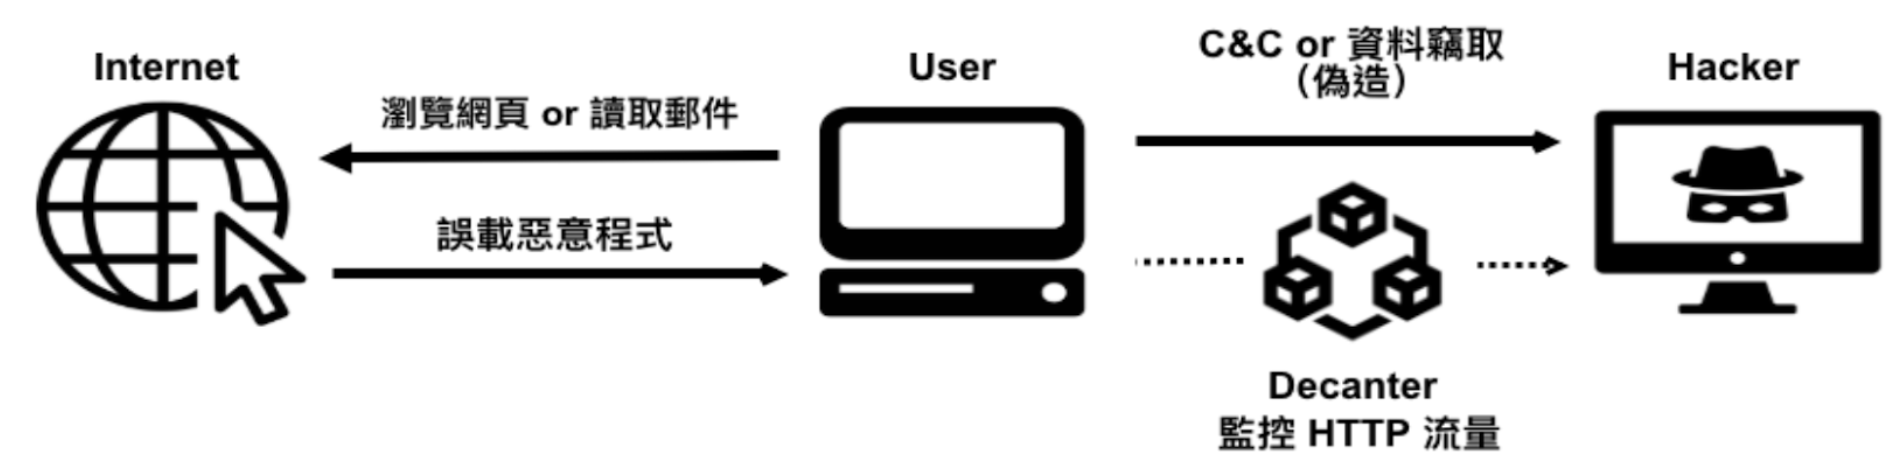
\includegraphics[width=250pt]{image/attack.png}
\caption{A process of attacking scenario}
\label{fig:attack}
\end{figure}

\begin{figure}[!tbp]
  \centering
  \subfloat[Normal Referrer Correlation Graph]{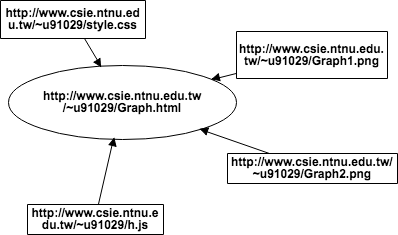
\includegraphics[width=0.4\textwidth]{image/normal.png}\label{fig:normal}}
  \hfill
  \subfloat[Malicious Referrer Correlation Graph]{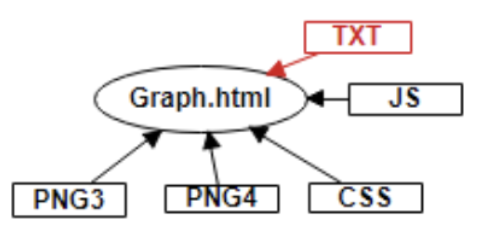
\includegraphics[width=0.4\textwidth]{image/malware.png}\label{fig:malware}}
  \caption{Difference between normal and malicious referrer correlation graph.}
\label{fig:length_count}
\end{figure}

To resolve this problem, we propose an approach based on deviation estimating when given referrer correlation graphs in training and testing phases, and the contributions of this work are briefly summarized as followings:

\begin{itemize}

\item We propose a solution to detect outbound anomalous HTTP connections, which is based on browser fingerprint and referrer correlation techniques. Furthermore, our approach automatically generates  fingerprints from network traffic, filter anomalous communications from the monitored hosts, and then identify counterfeit fingerprint in normal traffics which are filtered by fingerprints \cite{bortolameotti2017decanter}.

\item We proposed a counterfeit fingerprint detection to resolve counterfeit problem, which identifies fake contents of HTTP header based on graph edit distance. Besides, we also have implemented a system based on our approach in python, and the current state of the art regarding client-side anomaly detection which is already in collaboration with other institution and enterprise. 

\item We have evaluated and compared DECANTeR \cite{bortolameotti2017decanter} with real-world datasets. In the performance results, we show that our approach is better, especially the counterfeit fingerprint is harder to evade our approach.

\end{itemize}

In the remaining parts of this report, Section 2 surveys related work, and Section 3 describes the detail components of the proposed approach. The effectiveness, performance, and case studies of the proposed framework are evaluated and discussed in Section 4. At last, Section 5 concludes this project.
